\documentclass[a4j]{jsarticle}
\usepackage[dvipdfmx]{graphicx}
\usepackage{float} %表
%\usepackage{subfigure} %図を並べて表示しそれぞれのキャプションと全体のキャプションをつける
\usepackage{itembkbx}
\usepackage{eclbkbox} %改ページで枠を閉じない, ソースコードの枠
\usepackage{moreverb}
\usepackage{url} %URLをそのまま表示
\usepackage{amsmath, amssymb} %数式
%\usepackage{eqnarray} %数式, 複数行
\usepackage{multirow} %表縦結合のとき上下中央揃え
\usepackage{fancybox}%1行囲み
\usepackage{ascmac}%複数行囲み
\usepackage{listings,jlisting}
\usepackage{comment}
\lstset{%
  % language={c++},
  basicstyle={\small},%
  identifierstyle={\small},%
  commentstyle={\small\itshape},%
  keywordstyle={\small\bfseries},%
  ndkeywordstyle={\small},%
  stringstyle={\small\ttfamily},
  frame={tbrl}, %枠線
  breaklines=true,
  breakindent = 8.58pt,
  columns=[l]{fullflexible},%
  numbers=left,%
  xrightmargin=0zw,%
  xleftmargin=3zw,%
  numberstyle={\scriptsize},%
  stepnumber=1,
  numbersep=1zw,%
  lineskip=-0.0ex%
}%ここまでプログラムリストを表示するやつ

\title {工学実験実習III第3回\\スタックの実装と応用}
\author {15316 17番 竹村太希}
\date{実験日時:2018年6月15日, 2018年6月22日
\\ 提出日:\today}

\begin{document}
%タイトル    
\maketitle
\thispagestyle{empty}
\newpage
\setcounter{page}{1}
\pagestyle{plain}
%%

%==================== 概要 ====================%
\section{スタックの概要}
    スタックは, 食器棚に積まれた皿に例えられる. 洗い終わった皿は一番上に積まれ, 
    皿を使う際には一番上から取り出される.  
    このようにスタックには, 最後に入れたデータが一番最初に出てくる
    (逆を言えば, 最初に入ったデータは一番最後に出てくる)という特徴があり, LIFO(Last In First Out)型, または
    FILO(First In Last Out)型と呼ばれている. 

    スタックはしばしば, キューというデータ構造と比較される. キューはiPhone発売の際にApple Storeに夜通し
    列を作って並ぶ人々と同じで, 最初に並んだ人が最初にiPhoneを手に取ることができる. 
    身の回りでもよく見られる, 順番が守られている早いもの勝ちの世界である. 
    このようにキューは最初に入ったデータが最初に出てくる(逆を言えば, 最後に入ったデータは最後に出てくる)という特徴があり, 
    FIFO(First In First Out)型, またはLILO(Last In Last Out)型と呼ばれている. 
    
    \begin{figure}[H]
        \centering
        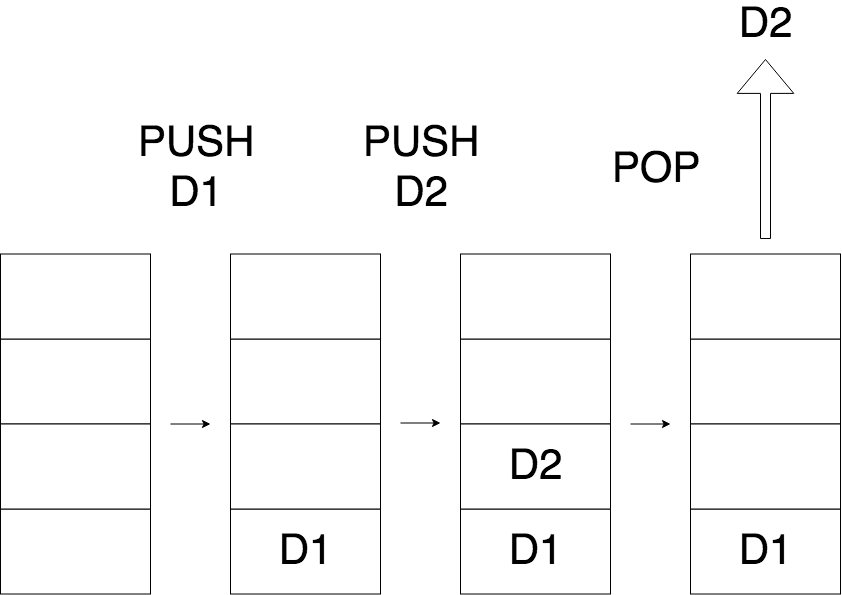
\includegraphics[scale=0.3]{stack.png}
        \caption{スタックのデータ構造}
        \label{stack}
    \end{figure}
%==================== 関数 ====================%
\section{スタックのための関数}
    スタックを実装するには, 実際にデータを格納するための配列と, 最後にデータを追加した位置より一つ上
    (次にデータを格納すべき場所)を指し示すポインタ, 
    そしてスタックを初期化するinit関数, スタックにデータを追加するpush関数, スタックからデータを取り出すpop関数
    があればよい. 今回はそれらに加えスタックの中身を表示するprintTower関数も作成する. 

    なお, 今回作成したスタックで扱えるデータ型は整数型のみとする. 

    \subsection{スタック構造体の定義}
    実際にデータを格納する整数型配列stack[]と, 最後にデータを追加した位置より一つ上の位置を格納しておく
    volume変数をセットにした構造体を定義する. 
    なお, 配列の大きさがスタックの深さ(つまりは食器棚の大きさ)となる. 今回は5段とマクロで定義した. 
    \begin{lstlisting}[label = s-1, caption = スタック構造体の定義]
#define HEIGHT 5


struct _Stack {
	int stack[HEIGHT];
	int volume;
};
typedef struct _Stack Stack;
    \end{lstlisting}

    \subsection{初期化関数}
    スタックとして使う配列stackの値を0に初期化し, 次にデータを格納すべき位置volumeを0番に設定する整数型関数initを作成. 
    引数には初期化するスタックのポインタを取った. 
    \begin{lstlisting}[label = init, caption = 初期化関数init]
int init(Stack *stack) {
	//スタックの格納配列の初期化
	for (int i = 0; i < HEIGHT; i++) {
		stack->stack[i] = 0;
	}
	//現在位置を0に設定
	stack->volume = 0;
	return 0;
}
    \end{lstlisting}

    \subsection{push関数}
    引数にスタックのポインタと追加するデータを取り, volumeにて示される位置にデータを追加するpush関数を作成. 
    \begin{lstlisting}[label = push, caption = push関数]
int push(Stack *stack, int num) {
	//Stack Overflow対策
	if (stack->volume >= HEIGHT) {
		return -1;
	}
	else {
		//引数で受け取った数を積み上げ
		stack->stack[stack->volume] = num;
		stack->volume++;
	}
	return 0;
}
    \end{lstlisting}
    \subsection{pop関数}
    スタックの一番上に格納されているデータを取り出してくる関数. 引数には取り出したいスタックの構造体のポインタを取る. 
    \begin{lstlisting}[label = pop, caption = pop関数]
int pop(Stack *stack) {
	//Stack Underflow対策
	if (stack->volume == 0) {
		return -1;
	}
	else {
		stack->volume--;
		int out = stack->stack[stack->volume];
		stack->stack[stack->volume] = 0;
		return out;
	}
}
    \end{lstlisting}
    \subsection{スタック表示関数}
    スタックのデータ格納状態を表示する. 引数には表示するスタックの構造体を取る.  
    \begin{lstlisting}[label = printstack, caption = スタック表示関数]
void printStack(Stack *stack) {
	for (int i = 0; i < HEIGHT; i++){
		printf("%d ", stack->stack[i]);
	}
	printf("\n");
}
    \end{lstlisting}
    
    
    
%==================== スタックの実行結果 ====================%
\section{実行結果}
    スタックにデータを追加していき, 正しく格納されたか調べると同時に, pop操作で正しく取り出されるか確認する. 
    なお, 確認するためにmain関数内を以下ソースコード\ref{stackmain}のように書いた. 
    \begin{lstlisting}[label = stackmain, caption = スタックの動作確認のためのmain関数]
int main() {
	struct Stack stack;

	init(&stack);
	push(&stack, 10); //10を追加
	push(&stack, 20); //20を追加
	push(&stack, 30); //30を追加
	push(&stack, 40); //40を追加
	push(&stack, 50); //50を追加
	printTower(stack);
	printf("%d\n", pop(&stack)); //50がpopされる
	printf("%d\n", pop(&stack)); //40がpopされる
	printf("%d\n", pop(&stack)); //30がpopされる
	printf("%d\n", pop(&stack)); //20がpopされる
	printf("%d\n", pop(&stack)); //10がpopされる
	return 0;
}
    \end{lstlisting}

    実行結果を実行結果1に示す. 
    %実行結果
    \begin{breakitembox}[l]{実行結果1: push, pop操作の実行結果}
    \begin{verbatim}

10 20 30 40 50
50
40
30
20
10
    \end{verbatim}
    \end{breakitembox}
このように, 無事にpush関数によって値がスタックに追加され, pop関数によって先に入った値が先に出てきていることが分かる. 

スタックオーバーフロー対策も施したので, 正しく実行されるか確認する. 今回作成したスタックは5段なので
, 6段目にデータをpushした際にエラーを吐くはずである. 

確認するためのmain関数は以下ソースコード\ref{overmain}とした. 
\begin{lstlisting}[label = overmain, caption = スタックオーバーフローの動作確認のためのmain関数]
int main() {
	Stack stack;

	init(&stack);
	push(&stack, 10); //10を追加
	push(&stack, 20); //20を追加
	push(&stack, 30); //30を追加
	push(&stack, 40); //40を追加
	push(&stack, 50); //50を追加
	printStack(stack); //既にこの時点で5段満杯となっている. 確認のため中身をすべて表示する. 
	push(&stack, 60); //更に追加しようとしてみる. 
	return 0;
}
\end{lstlisting}
実行結果を, 以下実行結果2に示す. 
\begin{breakitembox}[l]{実行結果2: スタックオーバーフローの実行結果}
\begin{verbatim}

10 20 30 40 50
ERROR: Stack overflow
\end{verbatim}
\end{breakitembox}
エラーを吐いているので, 正しくエラー処理が実行されたことが分かる. 

スタックアンダーフロー対策も施したので, 正しく実行されるか確認する. 確認するためのmain関数は以下ソースコード\ref{underflow}
とした. 
\begin{lstlisting}[label = underflow, caption = スタックアンダーフロー動作確認のためのmain関数]
int main() {
	Stack stack;

	init(&stack);
	push(&stack, 10); //10の追加
	push(&stack, 20); //20の追加
	printStack(stack); //一応格納されたかの確認
	printf("%d\n", pop(&stack)); //20をpop
	printf("%d\n", pop(&stack)); //10をpop
	printStack(stack); //この時点でスタックにデータが格納されていないことを確認
	pop(&stack); //更にpopを試みる
	return 0;
}
\end{lstlisting}
実行結果を, 以下実行結果3に示す. 
\begin{breakitembox}[l]{実行結果3: スタックアンダーフローの実行結果}
\begin{verbatim}

10 20 0 0 0
20
10
0 0 0 0 0
ERROR: Stack underflow
\end{verbatim}
\end{breakitembox}
エラーを吐いているので, エラー処理が正しく実行されたことがわかる. 

%==================== ハノイの塔作成の説明と実行 ====================%
\section{ハノイの塔}
    \subsection{ハノイの塔の概要}
        ハノイの塔とは, 積み重なった円盤を他の塔に, 少ない回数で移動させる手順を競うパズルゲームの一種である. 
        バラモンの塔, またはルーカスタワーとも呼ばれる. 
        
        3本の杭と, 中央に穴の開いた大きさの異なる複数の円盤から構成され, そのうち1本の杭に大きい円盤を下にして順に小さいものが上になるように
        積み重ねられている. 円盤を1回に付き1枚どれかの杭に移動させることができるが, 小さな円盤の上に大きな円盤を載せることはできない. 
    \subsection{この実験で取り組む意義}
        杭に円盤を重ねたり, 円盤を取り出したりする行為が最上位の円盤に対してのみ実行でき, LIFO型というスタックの
        構造に類似している. 
        
        そこで先に作成したスタックを用いてハノイの塔を作成することにより, スタックというデータ構造について理解を深める. 
    \subsection{ハノイの塔のための関数}
        ハノイの塔を作成するために, 新たに作成する関数を示す. 
        \subsubsection{移動チェック関数}
        移動元の塔から移動先の塔に移動可能かどうか判断する. 
        
        具体的には, 移動元の最上位の値が移動先の値よりも大きいことを確認する. 
        引数には移動元の塔の構造体と移動先の塔の構造体を, それぞれポインタとして取る. 戻り値には, 移動可能であれば1, 移動不可能であれば0を指定した. 
        
        実際に書いたソースコードを以下ソースコード\ref{hanoimove}に示す. 
        \begin{lstlisting}[label = hanoimove, caption = 移動チェック関数]
int enableStack(Stack *from_tower, Stack *to_tower) {
        if (from_tower->volume == 0) {
                return false;
        }
        if ((from_tower->stack[from_tower->volume - 1] < to_tower->stack[to_tower->volume - 1]) || to_tower->volume == 0) {
                //移動元のタワーの最上位の値が, 移動先の最上位の値より大きい もしくは移動先が
                return True;
        }
        else {
                return False;
        }
}
        \end{lstlisting}
        \subsubsection{完了チェック関数}
        ゲームがクリアされているのか, それともまだ継続するのかを判定する関数. 
        
        引数にはクリアしたかどうかチェックする構造体のポインタ, 設定した全ブロック数の2つを取る. 戻り地には, クリアしていれば1を, まだ継続する場合は0を指定した. 
        
        実際に書いたソースコードを以下ソースコード\ref{hanoiclear}に示す. 
        \begin{lstlisting}[label = hanoiclear, caption = 完了チェック関数]
int checkFinish(Stack *tower, int blocks) {
        //blocksは段数
        //すべての値が0になっているかチェック
        for (int i = 0; i < blocks; i++) {
                if (tower->stack[i] != 0) {
                        return False;
                }
        }
        return True;
}
        \end{lstlisting}
        
        
    \subsection{ハノイの塔プログラム}
    \begin{lstlisting}[label = hanoiAll, caption = ハノイの塔プログラム]
#include <stdio.h>
#include <stdlib.h>
#define HEIGHT 5
#define TOWERS 3
#define True 1
#define False 0

struct _Stack {
        int stack[HEIGHT];
        int volume;
};
typedef struct _Stack Stack;


int init(Stack *stack) {
        //スタックの格納配列の初期化
        for (int i = 0; i < HEIGHT; i++) {
                stack->stack[i] = 0;
        }
        //現在位置を0に設定
        stack->volume = 0;
        return 0;
}


int push(Stack *stack, int num) {
        //Stack Overflow対策
        if (stack->volume >= HEIGHT) {
                return -1;
        }
        else {
                //引数で受け取った数を積み上げ
                stack->stack[stack->volume] = num;
                stack->volume++;
        }
        return 0;
}


int pop(Stack *stack) {
        //Stack Underflow対策
        if (stack->volume == 0) {
                return -1;
        }
        else {
                stack->volume--;
                int out = stack->stack[stack->volume];
                stack->stack[stack->volume] = 0;
                return out;
        }
}


void printStack(Stack *stack) {
        for (int i = 0; i < HEIGHT; i++) {
                printf("%d ", stack->stack[i]);
        }
        printf("\n");
}


int enableStack(Stack *from_tower, Stack *to_tower) {
        if (from_tower->volume == 0) {
                return false;
        }
        if ((from_tower->stack[from_tower->volume - 1] < to_tower->stack[to_tower->volume - 1]) || to_tower->volume == 0) {
                //移動元のタワーの最上位の値が, 移動先の最上位の値より大きい もしくは移動先が
                return True;
        }
        else {
                return False;
        }
}


int checkFinish(Stack *tower, int blocks) {
        //blocksは段数
        //すべての値が0になっているかチェック
        for (int i = 0; i < blocks; i++) {
                if (tower->stack[i] != 0) {
                        return False;
                }
        }
        return True;
}


void printTower(Stack *towers, int blocks) {
        for (int i = 0; i < TOWERS; i++){
                printf("%d番目\t", i);
        }
        printf("\n========================\n");
        for (int i = blocks - 1; i >= 0; i--){
                for (int j = 0; j < TOWERS; j++) {
                        printf("%d\t", towers[j].stack[i]);
                }
                putchar('\n');
        }
}


int main() {
        int count = 1;
        int from_tower, to_tower;
        int tempNum;
        int blocks; //段数
        int flag;

        Stack towers[TOWERS];
        printf("段数を選んでください(3〜5): ");
        scanf_s("%d", &blocks);

        //初期化
        for (int i = 0; i < TOWERS; i++) {
                init(&towers[i]);
        }

        //第1塔に決められたブロックを積み重ね
        for (int i = blocks; i > 0; i--) {
                push(&towers[0], i);
        }

        printf("GAME START!\n");


        //ゲーム開始
        while (True){
                printf("[%d回目]\n", count);
                printTower(towers, blocks);
                printf("移動元と移動先を入力してください: ");
                scanf_s("%d %d", &from_tower, &to_tower);

                //存在しない塔への移動を弾く
                if (from_tower >= TOWERS || to_tower >= TOWERS) {
                        printf("存在しない塔が指定されました. リトライ\n");

                }
                //同じ塔から同じ塔に移動するのは無意味
                else if (from_tower == to_tower) {
                        printf("同じ塔の上で円盤が跳ねるだけで無意味. リトライ\n");
                } else {
                        if (enableStack(&towers[from_tower], &towers[to_tower]) == True) {
                                //移動可能なら移動
                                push(&towers[to_tower], pop(&towers[from_tower]));
                                count++;
                        } else {
                                printf("移動できません. やり直し\n");
                        }
                }
            
            //クリア判定
            if(checkFinish(&towers[0], blocks) && checkFinish(&towers[1], blocks)){
                printf("CLEAR!");
                break;
            }
            
            
        }
}

    \end{lstlisting}
    \subsection{実行結果}
        最短で移し終える動作の実行結果を実行結果4に示す. 
        \begin{breakitembox}[l]{実行結果4: ハノイの塔の実行結果}
        \begin{verbatim}

段数を選んでください(3〜5): 3
GAME START!
[1回目]
0番目   1番目   2番目
========================
1       0       0
2       0       0
3       0       0
移動元と移動先を入力してください: 0 2
[2回目]
0番目   1番目   2番目
========================
0       0       0
2       0       0
3       0       1
移動元と移動先を入力してください: 0 1
[3回目]
0番目   1番目   2番目
========================
0       0       0
0       0       0
3       2       1
移動元と移動先を入力してください: 2 1
[4回目]
0番目   1番目   2番目
========================
0       0       0
0       1       0
3       2       0
移動元と移動先を入力してください: 0 2
[5回目]
0番目   1番目   2番目
========================
0       0       0
0       1       0
0       2       3
移動元と移動先を入力してください: 1 0
[6回目]
0番目   1番目   2番目
========================
0       0       0
0       0       0
1       2       3
移動元と移動先を入力してください: 1 2
[7回目]
0番目   1番目   2番目
========================
0       0       0
0       0       2
1       0       3
移動元と移動先を入力してください: 0 2
CLEAR!
        \end{verbatim}
        \end{breakitembox}
        結果から, ハノイの塔のプログラムが正しく実行されることが読み取れる. 完了チェック関数も正しく実行されている. 
                
        なお, ルール上禁止されている動作を行おうとすると実行結果5のような結果となる. 
        \begin{breakitembox}[l]{実行結果5: ハノイの塔の実行結果}
        \begin{verbatim}

段数を選んでください(3〜5): 3
GAME START!
[1回目]
0番目   1番目   2番目
========================
1       0       0
2       0       0
3       0       0
移動元と移動先を入力してください: 1 2 [※虚無を移動することはできない]
移動できません. やり直し [*エラーメッセージ]
[1回目] [*移動ができない場合は回数を更新しない]
0番目   1番目   2番目
========================
1       0       0
2       0       0
3       0       0
移動元と移動先を入力してください: 0 5 [*存在しない塔へは移動できない]
存在しない塔が指定されました. リトライ
[1回目]
0番目   1番目   2番目
========================
1       0       0
2       0       0
3       0       0
移動元と移動先を入力してください: 0 0 [*同じ塔から同じ塔へ移動することは意味がない]
同じ塔の上で円盤が跳ねるだけで無意味. リトライ
[1回目]
0番目   1番目   2番目
========================
1       0       0
2       0       0
3       0       0
移動元と移動先を入力してください: 0 1
[2回目]
0番目   1番目   2番目
========================
0       0       0
2       0       0
3       1       0
移動元と移動先を入力してください: 0 1 [*小さい数の上に大きい数を重ねることはルール違反]
移動できません. やり直し
[2回目]
0番目   1番目   2番目
========================
0       0       0
2       0       0
3       1       0
移動元と移動先を入力してください:
...
        \end{verbatim}
        \end{breakitembox}
        このように, 移動チェック関数が正しく動作していることが分かる. 
%==================== 考察 ====================%
\section{考察}
    今回の実験を通して, スタックとは食器棚に皿を積んでいくようなものだと体験的に理解できた. また, スタックオーバーフローやスタックアンダーフロー
    といったエラーに対応することも出来るようになり, 実用性のあるスタックの実装が出来るようになった. さらにハノイの塔を通してスタックを使ったプログラムを書く体験もでき, これら大変将来に役立つ
    ことと思う. 
%==================== プログラム ====================%
\section{プログラム}
C言語で実装したスタックのプログラムを以下に示す. 
    \begin{lstlisting}[label = stackAll, caption = スタックのC言語による実装のソースコード]
#include <stdio.h>
#define HEIGHT 5


struct _Stack {
	int stack[HEIGHT];
	int volume;
};
typedef struct _Stack Stack;


int init(Stack *stack) {
	//スタックの格納配列の初期化
	for (int i = 0; i < HEIGHT; i++) {
		stack->stack[i] = 0;
	}
	//現在位置を0に設定
	stack->volume = 0;
	return 0;
}


int push(Stack *stack, int num) {
	//Stack Overflow対策
	if (stack->volume >= HEIGHT) {
		return -1;
	}
	else {
		//引数で受け取った数を積み上げ
		stack->stack[stack->volume] = num;
		stack->volume++;
	}
	return 0;
}


int pop(Stack *stack) {
	//Stack Underflow対策
	if (stack->volume == 0) {
		return -1;
	}
	else {
		stack->volume--;
		int out = stack->stack[stack->volume];
		stack->stack[stack->volume] = 0;
		return out;
	}
}


void printStack(Stack *stack) {
	for (int i = 0; i < HEIGHT; i++){
		printf("%d ", stack->stack[i]);
	}
	printf("\n");
}


int main() {
	Stack stack;
	init(&stack);

	push(&stack, 10); //10を追加
	push(&stack, 20); //20を追加
	push(&stack, 30); //30を追加
	push(&stack, 40); //40を追加
	push(&stack, 50); //50を追加
	printStack(&stack);
	printf("%d\n", pop(&stack)); //50がpopされる
	printf("%d\n", pop(&stack)); //40がpopされる
	printf("%d\n", pop(&stack)); //30がpopされる
	printf("%d\n", pop(&stack)); //20がpopされる
	printf("%d\n", pop(&stack)); //10がpopされる
	return 0;
}
    \end{lstlisting}
\end{document}
